\chapter{Humanoide Roboter}\label{sec:humanoide-roboter}
\section{Allgemein}\label{sec:allgemein}
Bei humanoiden Robotern handelt es sich um Roboter,
deren Zweck es ist, Menschen in Aussehen und Fähigkeiten nachzuahmen. Heute sind
Industrieroboter viel weiter verbreitet als humanoide Roboter und die Chance
z.~B. einen Mähroboter zu besitzen ist deutlich höher, als einen humanoiden
Roboter zu Hause zu haben. Wenn über das Thema Roboter im Allgemeinen gesprochen
wird, denken viele Menschen nichtsdestotrotz zuerst an humanoide Roboter oder
Androiden. \cite{Dautenhahn2011} 
%% XXX 
%% TODO
%% Schau mal alle XXX hier an. Das wirkt mir starkt nach Wiederholung

\subsection{Humanoide Roboter in Medien}
In vielen Science-Fiction Büchern, Serien und Filmen, sind Androiden oder
humanoide Roboter ein wesentlicher Bestandteil der Geschichte. Dabei treten sie
in sehr unterschiedlichen Arten auf. Jedoch haben alle gemeinsam, dass sie in
nicht all zu ferner Zukunft existieren und einen gewissen Einfluss auf das Leben
der Menschen haben. Dieser Einfluss ist in manchen Darstellungen positiv, in
anderen negativ.

\subparagraph{}
Geht es nach den Vorstellungen der Autoren,
scheint ein Leben ohne humanoide Roboter in Zukunft nicht vorstellbar zu sein.
Durch das häufige Auftreten in den Medien sind Androiden sehr weit in der
Vorstellung der Menschen vertreten. \cite{Dautenhahn2011}
%% XXX

\subsection{Faszination von humanoiden Robotern}
Obwohl Serviceroboter oder Industrieroboter technisch sehr aufwändig sein
können, haben sie für einen einzelnen Menschen meist keine sehr große Bedeutung.
Ein Mähroboter ist zwar nützlich, jedoch tut er von außen betrachtet nichts
anderes als den ganzen Tag über den Rasen zu fahren. Mit Industrierobotern
kommen Menschen noch seltener in Kontakt, wenn sie nicht gerade in einer Firma
arbeiten, in der diese eingesetzt werden. Auch diese Industrieroboter erledigen
meist nur eine einzelne Aufgabe und sind für Außenstehende auf Dauer wenig
interessant.

\subparagraph{}
Humanoide Roboter lösen hier eine viele größere Faszination aus. Sie
stellen eine Zukunftsvision dar, die in der Realität noch kaum vertreten ist.
Viele Menschen sind neugierig, was humanoide Roboter alles können und sind
fasziniert von ihren Fähigkeiten. Außerdem können Menschen mit humanoiden
Robotern interagieren. Sie können auf Fragen antworten, auf Berührungen
reagieren und die Menschen unterhalten. Dadurch sind humanoide Roboter auf
Dauer viel spannender als nicht interaktive Industrie- oder Serviceroboter.
\cite{Dautenhahn2011}
%% XXX

\section{Abgrenzung zu anderen Arten von Robotern}\label{sec:abgrenzung}
Häufig ist der Unterschied zwischen humanoiden Robotern und anderen Arten von
Robotern nicht ganz klar. So verschwimmen teilweise die Grenzen zwischen
Industrierobotern, Servicerobotern, humanoiden Robotern und Androiden.

\subsection{Industrieroboter}\label{sec:industrieroboter}
Der Unterschied zwischen humanoiden Robotern und Industrierobotern ist relativ
deutlich. Industrieroboter werden dazu entwickelt einzelne Schritte oder den
gesamten Fertigungsprozess zu automatisieren. Ihre Bewegungsabläufe erinnern oft
an die eines Menschen, da Industrieroboter meist aus mehreren Gelenken bestehen,
die unabhängig voneinander bewegt werden können, ähnlich wie der menschliche
Arm. \cite{Weber2017} Bei Industrierobotern wird allerdings kein besonderer
Fokus auf menschliche Bewegungen gelegt. Im Gegensatz zu humanoiden Robotern
werden Industrieroboter nicht entwickelt um einem Menschen ähnlich zu sein,
sondern um möglichst effizient arbeiten zu können.

\subsection{Serviceroboter}\label{sec:serviceroboter}
Unter Servicerobotern versteht man Roboter, die eine Aufgabe größten Teils
autonom erledigen. Bei diesen Aufgaben handelt es sich um Dinge, die ein Mensch
nicht erledigen kann oder will. Weit verbreitete Serviceroboter sind z.~B.
Staubsaugroboter oder Mähroboter. Der Unterschied zu humanoiden Robotern besteht
darin, dass Serviceroboter nur eine Art von Aufgaben erledigen können.
Außerdem ist ihr Aussehen an die zu erledigende Aufgabe angepasst, nicht an das
Aussehen eines Menschen.

\section{Moderne Humanoide Roboter}\label{sec:moderne-humanoide-roboter}
Trotz der weiten Verbreitung in Medien und der Vorstellung von
Menschen, machen humanoide Roboter nur einen kleinen Teil der Forschung
innerhalb der viel größeren Bereiche Robotik und Künstliche Intelligenz aus.
\cite{Dautenhahn2011} Trotzdem arbeiten verschiedene Unternehmen an der
Entwicklung von humanoiden Robotern und Androiden zum Einsatz in verschiedenen
Bereichen. Beipiele hierfür sind die im Folgenden vorgestellten Roboter.

\subsection{Atlas (Boston Dynamics)}
\begin{figure}
  \centering
     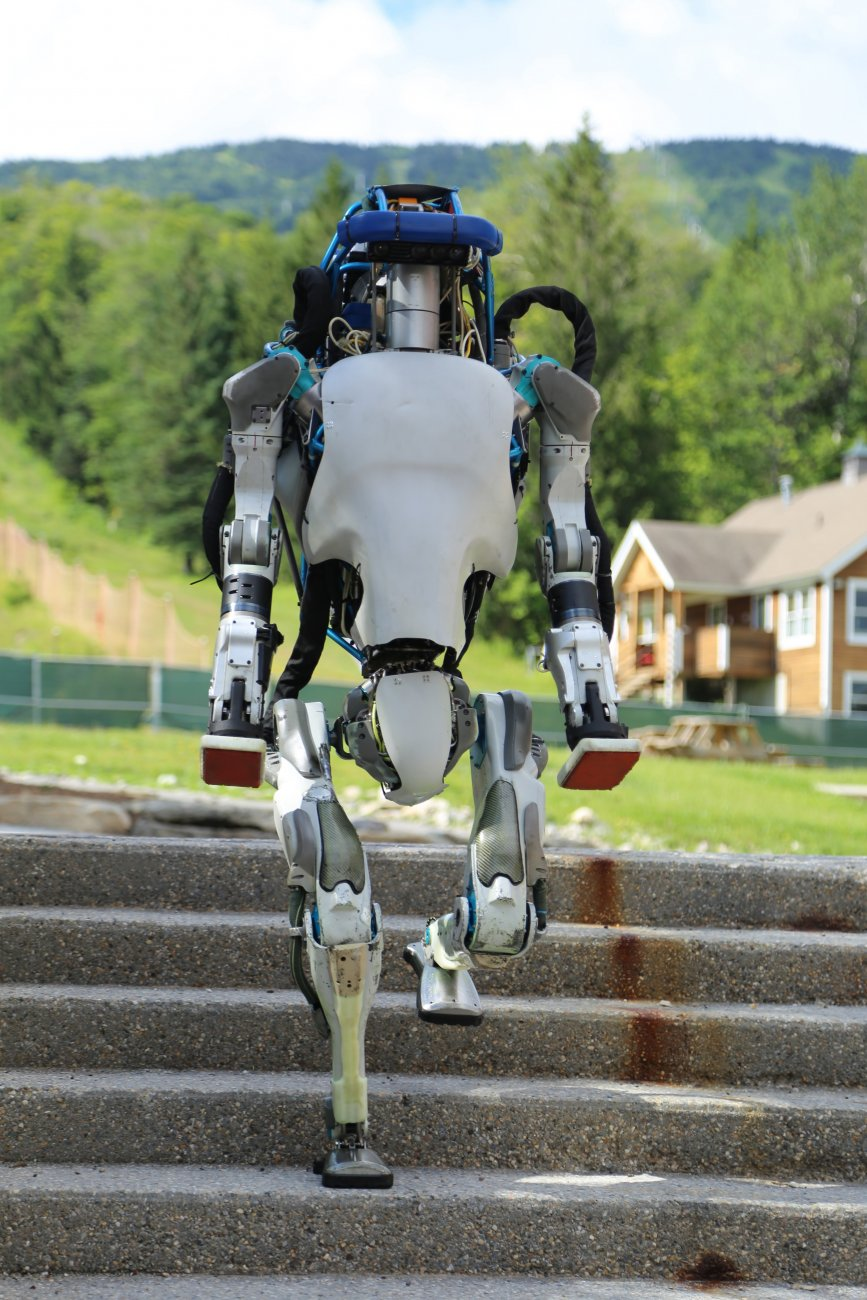
\includegraphics[width=0.5\textwidth]{atlas}
  \caption{Atlas \cite{AbbildungAtlas}}
  \label{fig:atlas}
\end{figure}
Atlas (Abb. \ref{fig:atlas}) wird von der Firma Boston Dynamics produziert.
Boston Dynamics ist bereits bekannt für seine laufenden Roboter, die sich auch
in unwegsamen Gebieten sicher fortbewegen können. Während andere Roboter von
Boston Dynamics Tieren nachempfunden sind, ist Atlas der erste Roboter der sich
wie ein Mensch bewegt und aussieht.

\subsection{Hub Robot (LG)}
\begin{figure}
  \centering
     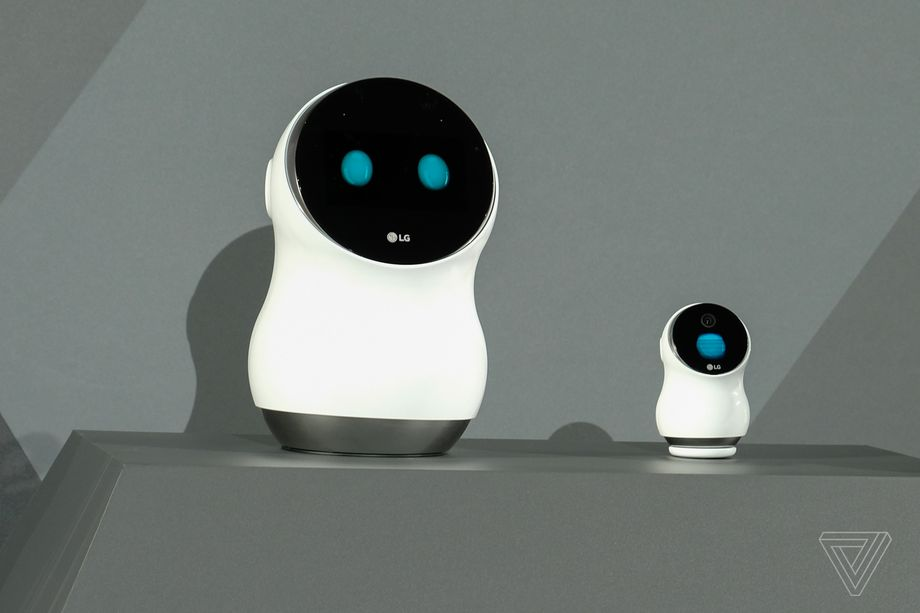
\includegraphics[width=0.7\textwidth]{hub_bot_privat}
  \caption{Hub Robot für Privatkunden \cite{AbbildungHubBotPrivat}}
  \label{fig:hub-bot-privat}
\end{figure}
\begin{figure} 
  \centering
     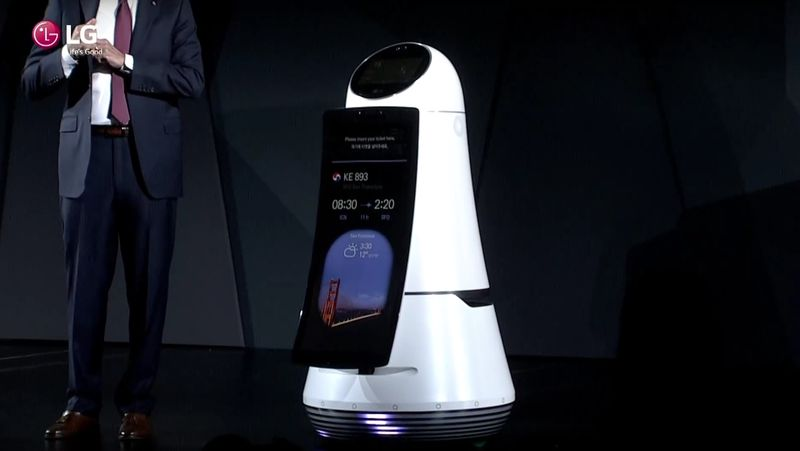
\includegraphics[width=0.7\textwidth]{hub_bot_firmen}
  \caption{Hub Robot für Firmenkunden \cite{AbbildungHubBotFirmen}}
  \label{fig:hub-bot-firma}
\end{figure}
LG präsentiert den Hub Robot in drei verschiedenen Varianten. Eine kleinere und
eine größere Version für Privathaushalte (Abb. \ref{fig:hub-bot-privat})
und eine noch größere Version, die zusätlich mit Rädern und einem zweiten
Display ausgestattet ist und an öffentlichen Plätzen, wie z.~B. Flughäfen
eingesetzt werden soll (Abb. \ref{fig:hub-bot-firma}). Der Hub Robot verwendet
Alexa von Amazon zur Sprachverarbeitung. Mit den beiden kleineren Varianten
lassen sich Smart Home Geräte steuern, welche LG ebenfalls anbietet. Außerdem
reagiert der Roboter mit seinem animierten Gesicht auf Emotionen der Personen,
die mit ihm interagieren. Die große Variante soll Passagiere an Flughäfen helfen
ihr Abfluggate zu finden und Informationen zu Flügen liefern. \cite{Patzschke2018}

\subsection{Paul (Fraunhofer-Institut)}
\begin{figure}
  \centering
     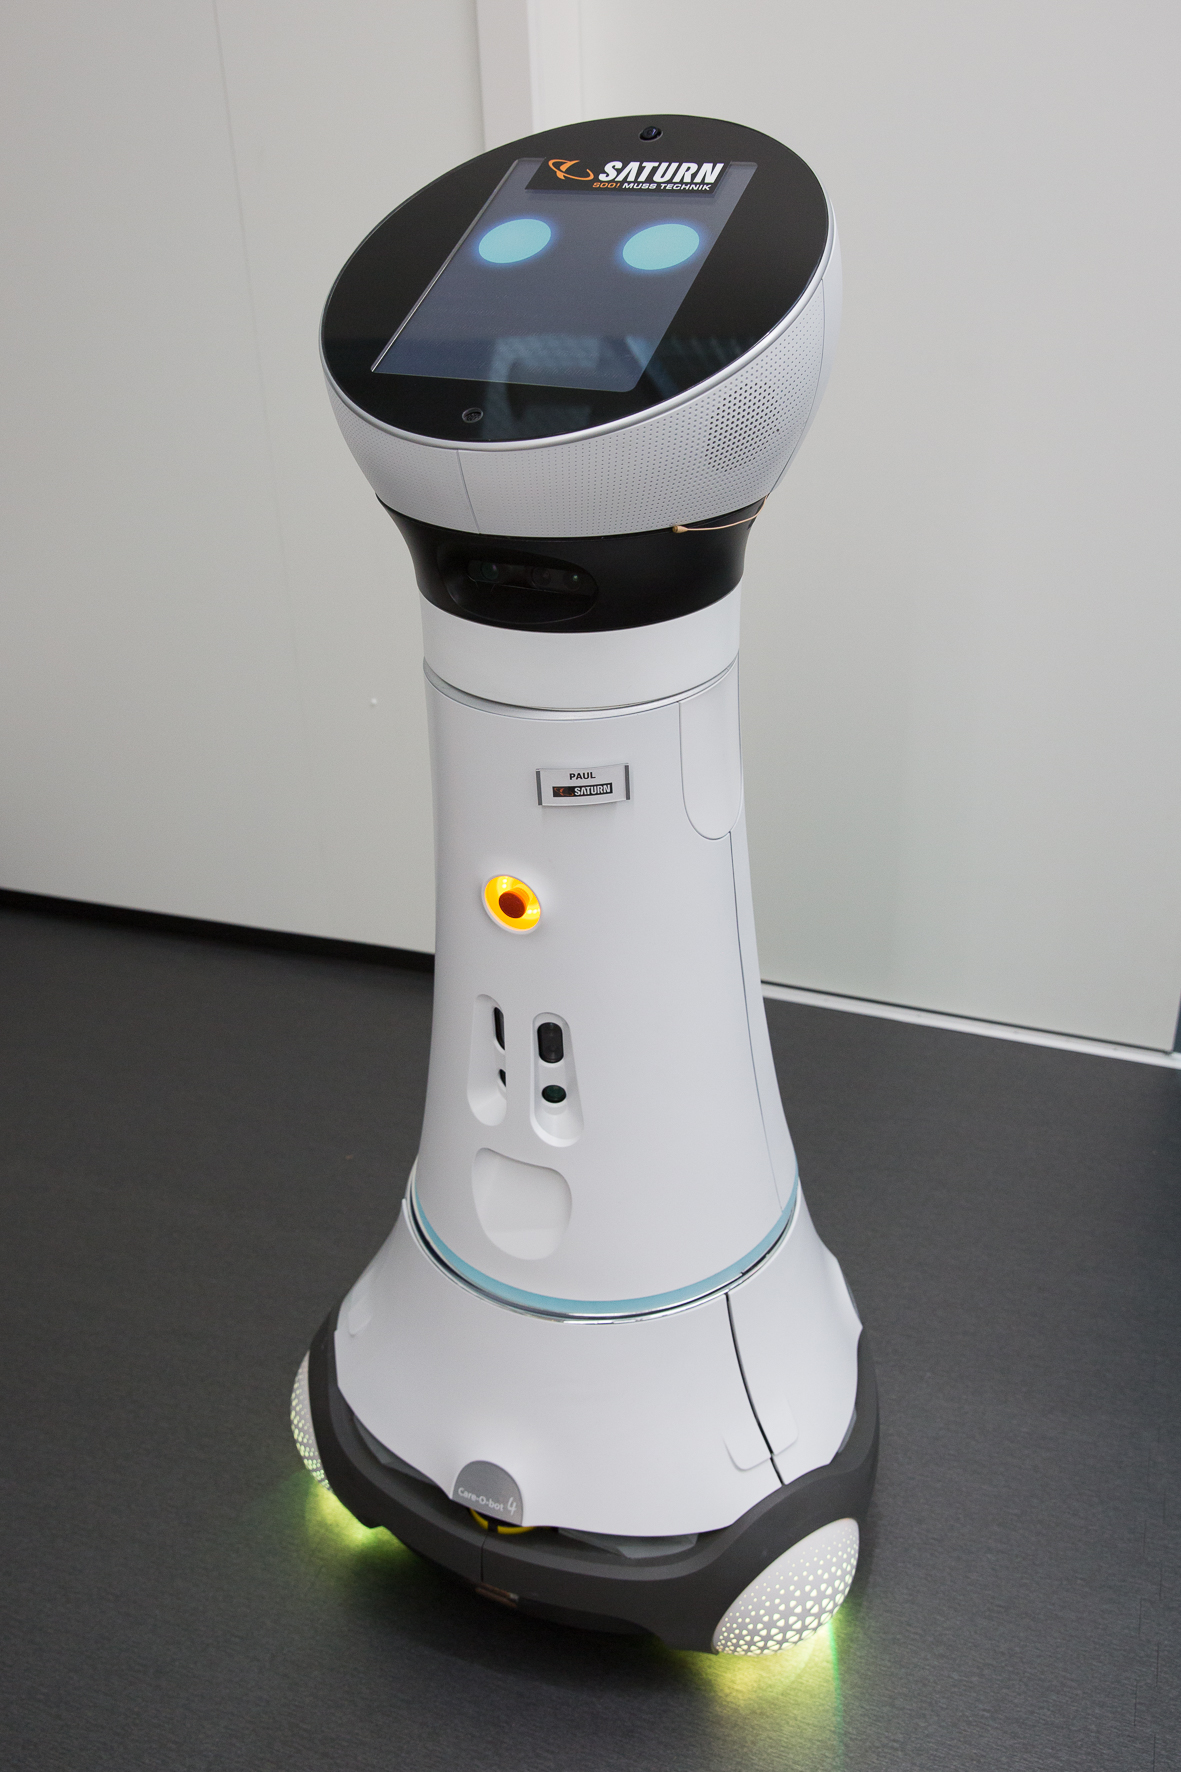
\includegraphics[width=0.5\textwidth]{paul}
  \caption{Paul \cite{AbbildungPaul}}
  \label{fig:paul}
\end{figure}
Paul (Abb. \ref{fig:paul}) ist eine Entwicklung des Fraunhofer-Instituts für
Produktionstechnik und Automatisierung. Der humanoide Roboter wird speziell für
den Einsatz im Handel angepasst. Paul verfügt über Produktinformationen eines
Marktes und kennt deren Standorte. So soll er Kunden zu einem Produkt begleiten
und ihnen Informationen liefern. Außerdem weißt er z.~B. auf Sonderaktionen des
Marktes hin. Um zusätzlich eine Attraktion zu sein, die Kunden anlockt, kann
Paul auch Smalltalk. \cite{MediaMarktSaturn2017}

\subsection{Sophia (Hanson Robotics)}
\begin{figure}
  \centering
     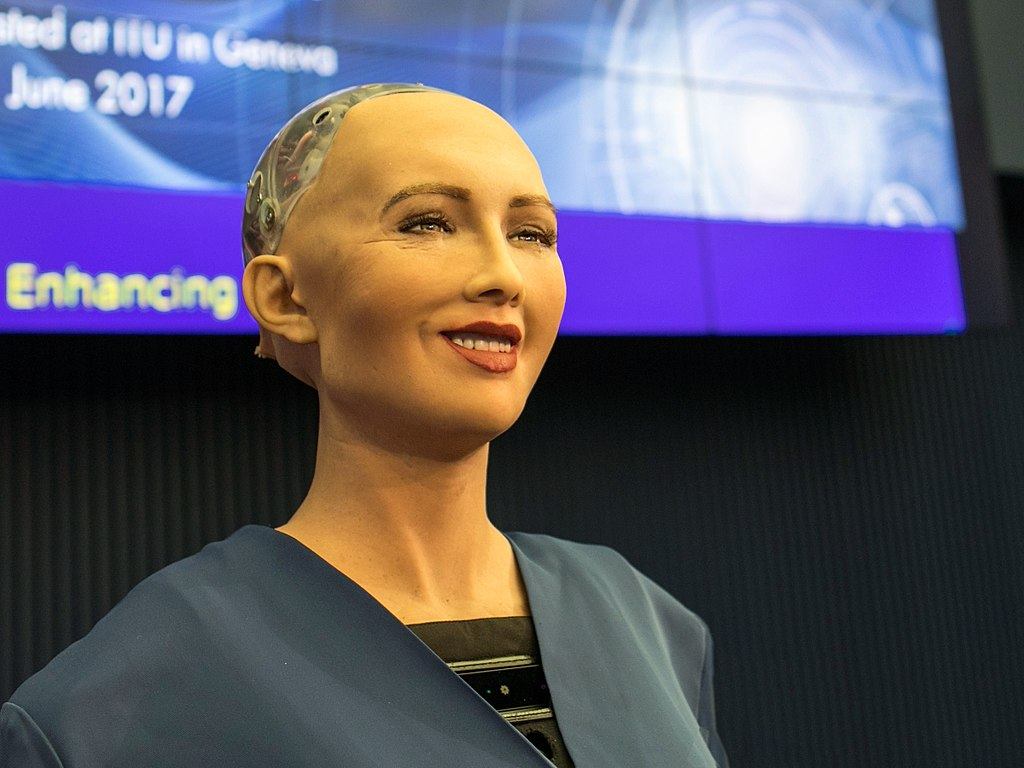
\includegraphics[width=0.5\textwidth]{sophia}
  \caption{Sophia \cite{AbbildungSophia}}
  \label{fig:sophia}
\end{figure}
Das Unternehmen Hanson Robotics arbeit daran den menschlichsten Roboter, der zur
Zeit existiert, zu entwickeln. Sophias Silikonhaut ist kaum von menschlicher
Haut zu unterscheiden (Abb. \ref{fig:sophia}). Der Roboter kann über 62
Gesichtsausdrücke darstellen.
Mit Kameras in den Augen, kann Sophia Menschen verfolgen und Augenkontakt zu
ihnen aufnehmen. Zusammen mit verschiedenen Technologien von Google, IBM und
Intel kann Sophia Sprache erkennen und sie verarbeiten. Außerdem lernt sie
dazu. \cite{Harriet2016} Auf der "`Future Investment Initiative"', einer
Konferenz in Saudi-Arabien wurde Sophia der Öffentlichkeit präsentiert. Dabei
wurde sie von einem Moderator interviewt. Das Gespräch mit Sophia wirkt
natürlich. Während dieser Konferenz wurde Sophia die arabische
Staatsbürgerschaft verliehen, dies ist allerdings eher als PR-Gag zu verstehen,
als dass Sophia soweit entwickelt ist, dass sie die Staatsbürgerschaft wirklich
verdient. \cite{Welt2017}

\subsection{Pepper (SoftBank Robotics und Aldebaran)}\label{sec:pepper}
\begin{figure}
  \centering  
     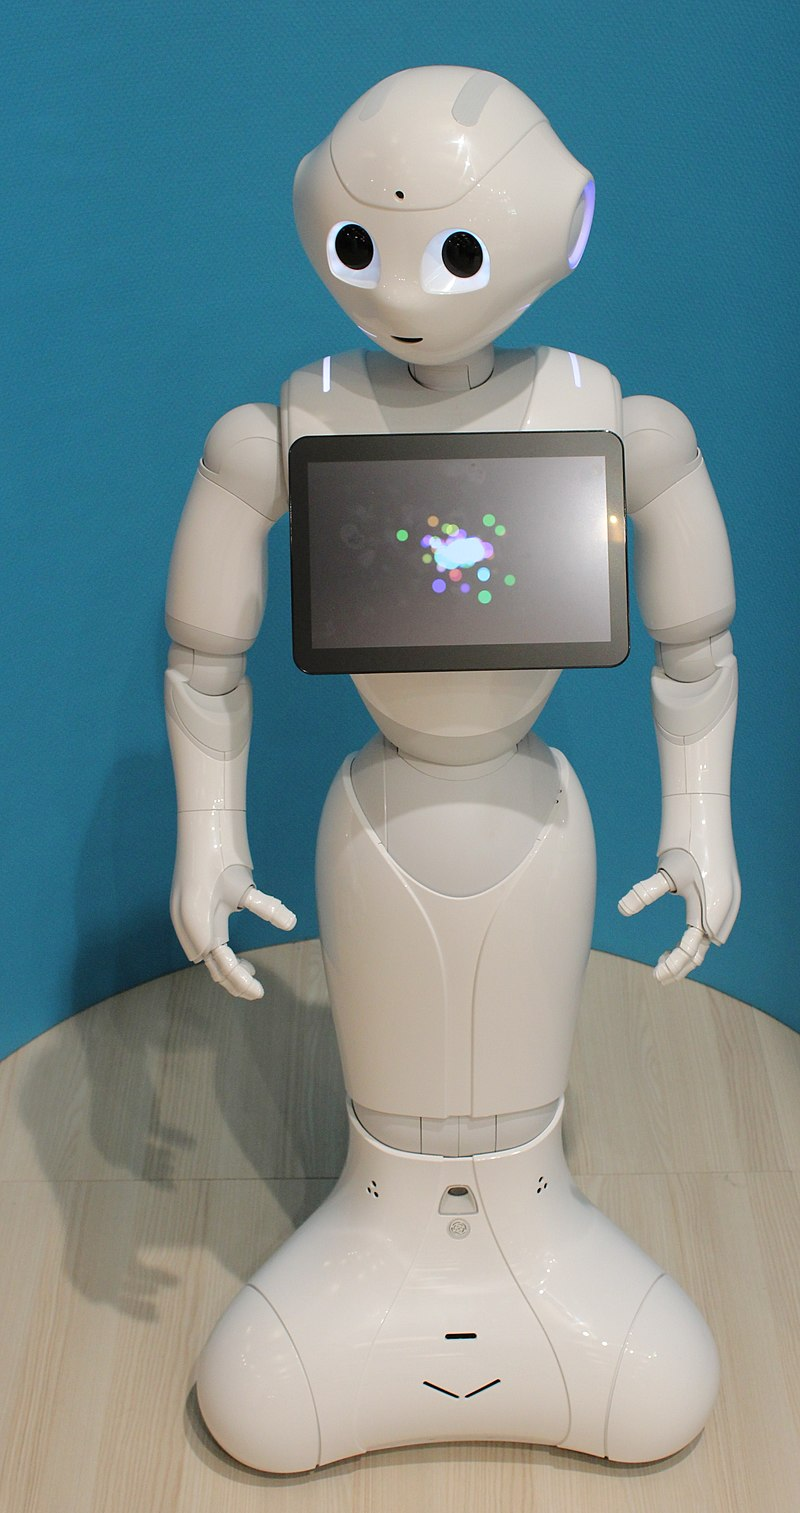
\includegraphics[width=0.4\textwidth]{pepper}
  \caption{Pepper \cite{AbbildungPepper}}
  \label{fig:pepper}
\end{figure}
Pepper (Abb. \ref{fig:pepper}) ist ein humanoider Roboter der Firmen SoftBank
Robotics und Aldebaran.
Vom Hersteller wird er als freundlich, liebenswert und überraschend beworben.
Entwickelt wurde Pepper um ein alltäglicher Begleiter für Menschen zu sein. Er
wird als "`viel mehr als ein Roboter"' beschrieben. Mit seiner Körpersprache und
der Stimme soll er auf die "`natürlichste und intuitivste"' Art mit Menschen
kommunizieren. \cite{SoftBank2018}

\subparagraph{}
Mit einer Größe von etwa 1,20m, seinem kindlichen Gesicht und beweglichen Armen
und Händen, soll Pepper Menschen glücklich machen. Sein Kopf bewegt sich, um
vorbeilaufende Passanten anzuschauen oder einem Menschen in die Augen zu
schauen, wenn er mit dem Roboter spricht. \cite{Markowitz2015}

\subparagraph{}
Das Design von Pepper ist darauf ausgelegt Emotionen sowohl zu verstehen als
auch auszulösen. Die dazu verwendeten Eigenschaften sind auch wichtig für das
Vorstellen von PowerPoint-Präsentation.

\subsubsection{Hören und Sprechen}\label{sec:hoeren-und-sehen}
Mit Lautsprechern und Mikrofonen ausgestattet, kann Pepper gesprochenes
Verstehen und darauf reagieren. \cite{SoftBankII2018} In der Anwendung soll
Pepper die Notizen einer PowerPoint-Präsentation vorlesen, wozu die Mikrofone benutzt werden. Die
Fähigkeit zuzuhören soll dazu verwendet werden Pepper während der Präsentation
Anweisungen geben können. Er soll auf Befehle wie "`Pause"' und "`Weiter"'
reagieren und die Präsentation entsprechend pausieren bzw. fortsetzen.

\subsubsection{Sehen}\label{sec:sehen}
Eine 3D-Kamera und zwei HD-Kameras helfen Pepper seine Umgebung zu analysieren
und Menschen und Bewegungen zu erkennen. \cite{SoftBankII2018} Während einer
Präsentation wird diese Fähigkeit, außer bei der schon vom Hersteller implementierten
Kollisionserkennung, nicht verwendet. Es wird nicht nötig sein spezielle Dinge
zu erkennen.

\subsubsection{Verbindung}\label{sec:verbindung}
Pepper verfügt über eine Internetverbindung. \cite{SoftBankII2018} Dies ist
wichtig, da die PowerPoint-Präsentation vor der Vorstellung durch Pepper nicht zuerst auf den
Roboter geladen werden soll. Die Informationen, wie die einzelnen Folien und der
zugehörige Text, sollen auf einem Server bereitgestellt werden, auf den der
Roboter zugreifen kann.

\subsubsection{Tablet}\label{sec:tablet}
Auf der Brust von Pepper ist ein Tablet angebracht, auf dem Bilder, Videos oder
Webseiten angezeigt werden können. \cite{SoftBankII2018} Auf diesem Tablet
sollen die einzelnen Folien der PowerPoint-Präsentation angezeigt werden.

\section{Human-Robot Interaction}\label{sec:hri}
\ac{hri} ist ein relativ neues, aber wachsendes Forschungsgebiet, welches sich
mit der Interaktion zwischen Menschen und Robotern befasst. Außerdem soll
herausgefunden werden wie Roboter am besten mit Menschen zusammenarbeiten
können. Dabei hat \ac{hri} nicht nur Einfluss auf die Wirtschaft, sondern auch
auf mögliche Arten der Beziehungen zwischen Menschen und Robotern. Deshalb
verbindet \ac{hri} verschiedene Wissenschaften, wie Psychologie und
Sozialwissenschaften mit Informatik und Robotik. Eines der Hauptziele von
\ac{hri} ist das Erforschen möglichst natürlicher Wege der Kommunikation
zwischen Menschen und Robotern. \cite{Dautenhahn2011}

\subparagraph{}
Um eine natürliche Kommunikation zwischen Menschen und Robotern zu ermöglichen,
müssen mehrere, von einem Benutzer potenziell verwendbare, Interfaces
bereitgestellt werden. Dabei werden klassische mit neueren Interfaces
kombiniert.

\subsection{Graphisches Interface}
Ein klassisches Interface zur Interaktion mit Maschinen sind graphische
Input-Output Schnittstellen. Wie bereits von der Kommunikation mit Computern
bekannt, könnte ein Roboter durch Eingaben mit Maus und Tastatur gesteuert
werden. Diese Form des Interfaces ist durch die weite Verbreitung von Computern
den meisten Menschen bekannt. Allerdings sind Maus und Tastatur keine
natürliche Art der Kommunikation. Dieses Interface kann durch die Verwendung
eines Touchscreens intuitiver und damit auch natürlicher gestaltet werden.

\subparagraph{}
Vorteil von graphischen Interfaces ist, dass der Benutzer dem Roboter klare
Instruktionen geben kann. über Menüs muss der Benutzer eine bestimmte Aktion
auswählen, die der Roboter ausführen soll. Der Roboter führt dann den
entsprechenden Programmcode aus. Auf diese Weise gibt es keinen Spielraum für
eventuelle Fehlinterpretationen der Instruktionen durch den Roboter.

\subsection{Sprache}
Sprache ist eine sehr natürliche Form der Kommunikation. Ein Mensch kann einem
Roboter einen Befehl geben, indem er dem Roboter sagt, welche Aktion er
ausführen soll. Der Mensch ist es gewohnt durch das Sprechen zu kommunizieren,
deshalb ist Sprache sowohl ein natürliches als auch ein intuitives Interface.

\subparagraph{}
Allerdings ist die Umsetzung dieses Interface komplizierter als die eines
einfachen graphischen Interface. Zunächst muss der Roboter die Worte, die der
Mensch spricht erkennen. Spracherkennung ist bereits weit verbreitet und wird in
verschiedenen Anwendungen verwendet. So lassen sich z.~B. Smartphones mit Siri
oder dem Google Assistant per Sprachbefehlen bedienen. Allerdings muss der
Roboter auch das verstehen, was der Mensch meint. Schon eine vermeintlich
einfache Anweisung, wie z.~B. "`Setz dich."' kann vom Roboter unterschiedlich
interpretiert werden. Er kann sich z.~B. entweder auf einen Stuhl oder auf den
Boden setzen.

\subparagraph{}
Zwar sind Sprachbefehle natürlicher und intuitiver als graphische Eingaben auf
einem Display, dem Menschen, der dem Roboter Anweisungen gibt, wird es jedoch
schwerer fallen seine Anweisungen so präzise zu formulieren, dass der Roboter
genau das tut, was er tun soll. Durch die Auswahl aus einem Menü wäre dies
einfacher.

\subparagraph{}
Außerdem muss der Roboter sich an die Dynamik, die sich aus einer Interaktion
ergibt anpassen. Kommunikation besteht meist nicht nur aus einem Befehl des
Menschen und der darauf folgenden Aktion des Roboters. Der Roboter kann
nachfragen, wenn ein Befehl nicht präzise genug formuliert wird und entsprechend
auf die Antwort des Menschen reagieren. Diese Frage-Antwort Dynamik muss der
Roboter verstehen und Antworten in den richtigen Kontext setzen.

\subsection{Visuelle Kommunikation}
Mit einer Kamera kann der Roboter Bewegungen, Gesten und Mimik eines Menschen
erkennen. So kann der Roboter mit der Hand gesteuert werden, reagieren, wenn ein
Mensch Blickkontakt zu ihm aufnimmt. So ist es auch möglich einem Roboter einen
Bewegungsablauf vorzumachen, den er dann wiederholen kann, was das Erklären
einer Aktion deutlich vereinfachen kann.

\subsection{Tastsensoren}
In der direkten Interaktion wird es auch zu
Berührungen zwischen Meschen und Robotern oder Robotern untereinander kommen. Um
dabei keine Schäden zu verursachen oder Menschen zu verletzen muss der Roboter
auf Berührungen reagieren können. Berührungen sind eine direkte Form der
Kommunikation, die dem Roboter unmissverständlich bestimmte Anweisungen geben
kann. So kann fest einprogrammiert werden dass sich der Roboter nicht mehr
bewegt, nachdem er berührt wurde. Damit wird verhindert, dass er Menschen
verletzt. \cite{Prassler2004}

\section{Einsatz von humanoiden Robotern}\label{sec:einsatz}
\subsection{Öffentliche Plätze}\label{sec:oeffentliche-plaetze}
Im Incheon Internation Airport in Südkorea werden mehrere humanoide Roboter von
LG eingesetzt um für mehr Sauberkeit und eine leichtere Orientierung der
Passagiere zu sorgen. Dazu werden zwei verschiedene Typen von Robotern
verwendet. Zum einen ein Staubsaugroboter, der mit künstlicher Intelligenz
ausgestattet ist. Er merkt sich welche Bereiche am häufigsten gereinigt werden
müssen und berechnet so ideale Putzrouten.

\subparagraph{}
Zum anderen wird eine größere Variante des, auch für Privathaushalte
verfügbaren, "`Hub Robot"' verwendet. Dieser kann mit Passagieren kommunizieren
und über ein großes Display Informationen anzeigen. Bei Bedarf kann er Fluggäste
persönlich zu einem von ihnen gewählten Zielpunkt begleiten.
\cite{Beineke2017}

\subparagraph{}
Als erster deutscher Flughafen testet der Flughafen München zusammen mit
Lufthansa den Einsatz eines humanoiden Roboters. Dazu wird Pepper, vom Flughafen
"`Josie Pepper"' getauft, verwendet. In einer Testphase wird der Roboter im
Terminal eingesetzt. Es soll herausgefunden werden, wie die Reaktion der
Passagiere auf den Roboter ausfallen. Mit Hilfe von IBM Watson ist Pepper an
Daten des Flughafens angebunden und kann so Fragen der Passagiere beantworten.
So kann der Roboter zum Beispiel den Weg zum Abfluggate eines Fluges erklären.
\cite{MunichAirport2018}

\subparagraph{}
Ähnlich wie am Flughafen werden humanoide Roboter auch an Bahnhöfen eingesetzt.
In Frankreich wird Pepper an drei verschiedenen Bahnhöfen verwendet, um Reisende
während Wartezeiten zu unterhalten. Außerdem liefert Pepper Informationen zu
Zügen und erfasst die Kundenzufriedenheit. \cite{SoftBankIV2018}

\subsection{Einzelhandel}
Da humanoide Roboter Aufmerksamkeit auf sich ziehen, werden sie gerne verwendet,
um Kunden in Läden zu locken, sie auf Produkte hinzuweisen oder dafür zu sorgen,
dass Kunden sich länger im Laden aufhalten. Zum Beispiel wird Pepper in
Fillialen des Herstellers von Pepper, SoftBank, eingesetzt. Außerdem berät
Pepper Kunden in Fillialen von Nestlé in Japan und Carrefour in Frankreich.
\cite{SoftBankIV2018}

\subparagraph{}
Auch in deutschen Geschäften werden bereits Roboter
eingesetzt. So setzt Edeka ebenfalls auf den Roboter Pepper. Saturn und
Mediamarkt setzen Paul ein. Zur Zeit
müssen die Positionen der Artikel zu denen Pepper und Paul die Menschen führen
sollen noch manuell von Mitarbeitern eingegeben werden. Allerdings arbeitet das
Fraunhofer-Institut daran, für diese Aufgabe einen zweiten Roboter zu
entwickeln. \cite{Hildebrand2017}

\subsection{Körperlich anspruchsvolle und gefährliche Aufgaben}
Der Roboter Atlas wird entwickelt um sich selbständig durch unwegsames Gelände
bewegen zu können. Durch seine Bewegungsfähigkeiten, die denen des Menschen
ähneln, lässt er sich für Aufgaben einsetzen, die bisher von Menschen ausgeführt
wurden. Er kann zum Beipiel das Aufheben
und Tragen von schweren Gegenständen in Lagern oder auf Baustellen übernehmen.
Außerdem kann Atlas bei Bombenentschärfungen oder während Naturkatastrophen
eingesetzt werden. Damit können Atlas oder andere Roboter mit ähnlichen
Fähigkeiten Aufgaben übernehmen, die für Menschen zu gefährlich oder körperlich
zu anspruchsvoll sind. \cite{Kaczmarek2016}

\subsection{Pflege}
In Senioren- und Pflegeheimen ist Fachkräftemangel bereits heute ein Problem,
welches sich in Zukunft aufgrund des demographischen Wandels noch verstärken
wird. Humanoide Roboter können das Pflegepersonal in ihrer Arbeit unterstützen.
Die Universität Siegen arbeit daran den Roboter Pepper so weiterzuentwickeln,
dass er die Senioren unterhalten kann während Pflegekräfte mit anderen Aufgaben
beschäftigt sind. So soll Pepper Gedächtnis-Spiele mit den Bewohnern des
Seniorenheims spielen, Bewegungen vorführen und gute Laune verbreiten. \cite{Frei2017}

\subsection{Private Haushalte}
Außer als Spielzeug, werden humanoide Roboter in privaten Haushalten bisher
selten eingesetzt.
Als digitale Assistenten werden hauptsächlich Geräte wie \emph{Amazon Echo} oder
\emph{Google Home} verwendet. Diese sind über das Internet mit Smart Home
Geräten verbunden. Auf diese Weise lassen sich diese Geräte mit Sprachsteuerung
bedienen. Das führt dazu, dass kein humanoider Roboter nötig ist um Aufgaben wie
"`Schalte das Licht aus"' oder "`Stelle die Heizung an"' zu erledigen. Da
humanoide Roboter um einiges teurer sind, als digitale Assistenten, besteht für
Kunden kein Anreiz einen Roboter zu kaufen.

\subparagraph{}
Verschiedene Unternehmen setzen darauf, Roboter mit Emotionen auszustatten. Sie
können z.~B. ihren Kopf bewegen, Gesichtsausdrücke nachstellen oder tanzen wenn
sie "`glücklich"' sind. So wecken diese "`sozialen"' Roboter Emotionen in
Menschen. Dies ist ein Unterschied zu anderen digitalen Assistenten, welcher
Kunden dazu bewegen kann, sich einen Roboter zu kaufen. Auch wenn solche
Roboter bereits entwickelt wurden, sind sie zur Zeit kaum in privaten Haushalten
vertreten. Die Hersteller arbeiten jedoch daran Roboter weiterzuentwickeln. So
besteht die Möglichkeit, dass in Zukunft immer mehr Roboter Teil des Smart Homes
werden. \cite{Bager2018}
